\documentclass{subfiles}
\begin{document}
\begin{figure}[h!]
    \centering
    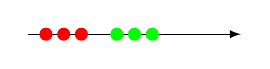
\begin{tikzpicture}[every node/.style={scale = 0.5},scale = 0.45]

        \draw [-latex] (-2, 0) -- (4, 0);

        \node (r1) at (-0.5, 0) [circle, fill = red] {};
        \node (r2) at (-1, 0) [circle, fill = red] {};
        \node (r3) at (-1.5, 0) [circle, fill = red] {};


        \node (g1) at (0.5, 0) [circle, fill = green] {};
        \node (g2) at (1, 0) [circle, fill = green] {};
        \node (g3) at (1.5, 0) [circle, fill = green] {};

    \end{tikzpicture}
    \caption{Effetto della PCA}
    \label{fig:2}
\end{figure}
\end{document}